%!TEX root = these.tex

\chapter[Exploration interactive de données moléculaire en immersion]{Naviguer et visualiser de façon naturelle et immersive}
\label{Sec:CantorDigitalis}
\minitoc
\cleardoublepage

Etape explicite de la boucle de biologie structurale (voir Figure \ref{Fig:schema_seq_bio_struct}), la visualisation de modèles 3d de protéines ou de complexes moléculaires permet à l'expert d'extraire de nombreuses informations de façon intuitive et rapide. Le rôle de la visualisation moléculaire pour communiquer et comprendre la biologie moléculaire a été mise en avant récemment \cite{}.
Nous avons cité plusieurs techniques de visualisation moléculaire dans la section \ref{visu_molecular} permettant de mettre en avant des informations structurelles ou physico-chimiques d'un simple coup d'oeil. Bien que ces informations soient déjà relativement complètes dans des environnements standards, elles peuvent être significativement améliorées par l'ajout de la profondeur dans la perception visuelle des données moléculaires. La RV et les technologies s'y rapportant permettent de rajouter cette 3e dimension grâce aux environnements virtuels (EV) et ainsi permettre une exploration plus naturelle des données.

Cependant, nous avons mis en exergue le frein que constitue la conscience spatiale altérée de l'utilisateur lors de l'exploration de complexes moléculaire dans des conditions immersives. Au-delà de la limitation spatiale que cela impose à l'utilisateur, cette conscience spatiale dégradée entraîne un malaise réduisant significativement la qualité de l'expérience de l'utilisateur. 

Pour répondre à ces problèmes issus directement de la RV, de nombreuses études ont été effectuées. Ces études sont cependant exclusivement réservées pour l'exploration de mondes virtuels écologiques, les études de navigation dans les données abstraites et scientifiques sont quant à elles beaucoup plus rares. 

Nous détaillerons tout d'abord dans ce chapitre notre approche pour répondre à l'évolution des moyens de partager des informations de structure moléculaires dans le monde scientifique. Nous analyserons ensuite les méthodes de navigation dans des scènes écologiques pour identifier les progrès à réaliser dans les scènes de données abstraites. Finalement nous présenterons nos développements et apport pour répondre au besoin de paradigmes de navigation adaptés aux données moléculaires.

\section{Les images stéréoscopiques au service de la visualisation moléculaire}

Nous avons souligné dans le chapitre 2 l'importance que prenait la visualisation et la représentation de structures 3d de molécules pour la compréhension de leur fonctionnement. En plus de permettre d'appréhender leur rôle biologique, la visualisation moléculaire est également un excellent vecteur de communication dans le monde scientifique. Fort de ce constat, nous nous sommes intéressés aux améliorations possibles que nous pourrions apporter aux moyens de communication actuels qu'offre la visualisation moléculaire. Ces derniers se concentrent exclusivement autour de l'échange de représentations graphiques générés par un certain nombre de logiciels experts comme PyMol, VMD ou YASARA pour ne citer qu'eux. Un rendu en deux dimensions d'une vue sur une partie ou l'ensemble d'une molécule permet, avec ou sans légendes appropriées, permet de rendre compte d'un phénomène ou d'une singularité structurelle précise. Si cette singularité est structurelle, elle est par définition 3d et pourrait donc être rendue de façon plus précise par un rendu 3d.

\subsection{L'évolution des méthodes de communication du monde scientifique}

Les moyens de communication scientifique se sont, en parallèle des moyens de communication standards, développés sur les appareils mobiles type smartphone et tablettes. Les journaux physiques et papiers sont de plus en plus rares au sein des labos et la grande majorité des articles scientifiques sont numérisés et accessibles en ligne. Le support a quelque peu évolué et une publication d'un article scientifique, en ligne ou non, suit les mêmes standards de format, majoritairement PDF contenant du texte et des images 2d. Quelques évolutions notoires sont apparues afin d'enrichir les contenus et les rendre interactifs \cite{attwood2010utopia}. Les structures moléculaires peuvent retrouver une 3e dimension grâce à plusieurs méthodes \cite{kumar2008grasping,raush2009new} qui dépendant cependant de pré-requis logiciels minimums pour être complètement fonctionnels ou requièrent des programmes spécifiques (comme la version 3d améliorée d'Adobe Acrobat reader\footnote{\url{http://get.adobe.com/reader/}} ou les plugins spécifiques comme le navigateur ICM\footnote{\url{http://www.molsoft.com/icm_browser.html}}).

En 1994, Green présenta le concept de <<stereoimages>> \cite{green_stereoimages_1994} pour les structures moléculaires. Basées sur la simple décomposition en deux vues, une pour l'oeil droit et une pour l'oeil gauche, de la représentation d'une molécule, elle permet d'avoir une perception 3d de la structure de façon simple et rapide. Nous avons mis à jour cette proposition à la lumière des nouvelles technologies désormais largement disponibles que sont les smartphones et les tablettes. Ces dispositifs mobiles offrent davantage de possibilités pour afficher du contenu scientifique et interagir avec lui facilement et de façon esthétique. Il semble ainsi qu'un décalage dans les habitudes de lecture d'articles scientifiques se fasse. Les éditeurs scientifiques ont d'ailleurs rapidement commencer à publier sur les périphériques mobiles: Cell Press\footnote{\url{http://www.cell.com/journalreader}}, ACS\footnote{\url{http://pubs.acs.org/page/tools/acsmobile/index.html}}, Nature Publishing\footnote{\url{http://www.nature.com/mobileapps}}, Science\footnote{\url{http://content.aaas.org/mobile}} ou PloS\footnote{\url{blogs.plos.org/everyone/2010/09/16/plos-reader-2-0/}} fournissent des application mobiles dédiées pour leurs publications. De la même manière, parmi les nombreuses applications dédiées à la procrastination, certaines se révèlent avoir une utilité scientifique significative \cite{powell_lab_2012}. On retrouve des applications de visualisation 3d de biomolécules, de visualisation 2d de petites molécules, des applications de calcul de masse molaire ou des applications informatives comme un tableau périodique. On retrouve parmi ces applications mobiles "scientifiques" une simplicité commune et des qualités de graphismes modestes, principalement dues aux puissances graphiques matériellement limitées des périphériques mobiles. Il est ainsi compliqué de permettre un rendu 3d complet d'un complexe moléculaire de taille raisonnable sur ces appareils. 

\subsection{DepthMol3d}

Il est cependant possible d'utiliser la puissance graphique, même restreinte, des smartphones/tablettes pour créer une perception 3d améliorée de systèmes moléculaires. C'est le but du développement de notre application, DepthMol3d, basé sur le moteur de jeu Unity3D\footnote{\url{http://unity3d.com/}}. Cette approche offre de nombreuses opportunités pour la recherche, la communication, la discussion et le monde de l'éducation.

\subsubsection{Ajouter la 3e dimension à une scène moléculaire}

Notre approche se base sur l'utilisation d'images 2d, beaucoup plus légères que des modèles 3d et permettant un certain degré de personnalisation de la part des utilisateurs. Indépendante de logiciels experts de visualisation, notre méthode ne nécessite qu'un périphérique mobile pour fonctionner et expérimenter l'effet 3d. Un nombre important de visualiseurs moléculaires peuvent être utilisés pour générer du contenu, VMD, Chimera, PyMol ou Yasara ont par exemple été utilisé pour générer plusieurs scènes exemples.

Deux images sont nécessaire pour parvenir à un effet 3d, une image de \textbf{texture} et une \textbf{carte de profondeur} (cf. Figure \ref). L'image de \textit{texture} est une capture de la scène 3d moléculaire. La \textit{carte de profondeur} possède elle les informations de profondeur pour l'image de texture à travers un gradient de couleur grise. Ce gradient de gris correspond à la distance entre chaque point de l'objet 3d et l'écran. Plus un objet est distant de la caméra (ou de l'écran d'ordinateur) et plus la couleur est sombre. Une fois que les deux images ont été générées, elles doivent être transférées sur le périphérique mobile où elles sont lues et traitées par notre application. Un navigateur de fichier intégré permet à l'utilisateur de trouver ses images et de les charger. Le principe d'une telle application est de créer un objet 3d à partir de la carte de profondeur dont la surface sera ensuite colorée par la texture associée (\ref{}). Avec ces données, l'application crée l'illusion d'une 3e dimension en ajoutant aux objets une sensation d'espace et de profondeur qui s'étend loin derrière l'écran. Cela est rendu possible par les calculs permanents de la direction de vue basée sur l'orientation du périphérique, mesurée par un accéléromètre ou un gyroscope embarqués dans la majorité des périphériques mobiles d'aujourd'hui, amenant à la sensation de regarder à l'intérieur d'une boîte qui s'étendrait derrière la surface d'écran de l'appareil.

\subsubsection{Explorer des modèles 3d de molécules}

Un deuxième mode de visualisation permet d'importer directement des mesh 3d dans DepthMol3d. Avec ce type de données 3d, seul un fichier est nécessaire pour créer une perspective 3d. Après importation, il est possible de manipuler l'objet, de le tourner, le déplacer en avant ou arrière. Cette visualisation se rapproche de ce qui peut se retrouver dans les visualiseurs moléculaires pour périphériques mobiles à ceci près que l'utilisateur aura également la possibilité de changer l'échelle de la molécule et de plonger à l'intérieur. Il utilisera alors son périphérique comme une fenêtre sur le monde virtuel, à la manière de ce que proposent de nombreux acteurs de la RV aujourd'hui n'ayant pas franchi le pas de la conception de casques de RV mais fournissant des supports type casque permettant de positionner un smartphone devant les yeux et de rendre une image stéréoscopique grâce à deux lentilles intégrées au support. L'exemple le plus connu est le \textit{cardboard} de Google permettant de mettre un smartphone d'environ 5 pouces de diagonale au sein d'un support en carton pliable comportant un jeu de lentille. Basés sur le gyroscope du périphérique, un simple mouvement de tête permet de regarder une zone différente de la molécule (voir Figure \ref).

\section{Navigation dans des données écologiques ou scientifiques}

La navigation dans des environnements virtuels 3d possède un certain degré de similitude avec la navigation dans le réel. La différence principale entre la navigation dans les espaces réel et virtuel se situe au niveau des modes/techniques de navigation qui sont propres à chaque réalité. La navigation est un concept très vaste qui nécessite dans un premier temps une clarification terminologique. Darken et Peterson (2002), spécialistes en cognition spatiale, remarquent qu'une confusion apparaît dans la littérature sur les termes employés. Ainsi, certains auteurs emploient comme synonyme les termes de « navigation », « déplacement » ou encore « exploration ». Ces trois termes sont au centre de la présente recherche d’où l’importance de définir clairement ces mots-clés. 
La navigation dans des environnements réels ou virtuels se définit à la fois par des composantes \textbf{motrices} et à la fois par des composantes \textbf{cognitives} \cite{bowman_doug_a_3d_2002}.

\begin{itemize}
	\item La composante motrice définit le mouvement/déplacement réel d’un utilisateur dans l’espace. Il existe plusieurs modes ou techniques de déplacement. Bowman (2002) les classe en deux catégories, selon la métaphore employée pour se déplacer dans l’espace virtuel :
		\begin{itemize}
			\item Les métaphores réelles qui font appel à des comportements réalistes et/ou naturels comme le déplacement en mode « marche », « vol », « à vélo » ou encore « en conduisant ».
			\item Les métaphores « virtuelles » où les chercheurs utilisent le potentiel du virtuel pour imaginer et créer des modes de déplacement dans l’espace. Ainsi, ces métaphores permettent de s’extraire des contraintes physiques. Elles demandent par conséquent l’apprentissage de leur fonctionnement. Parmi ces métaphores dites « virtuelles », on peut citer la téléportation (on spécifie les coordonnés de la cible à atteindre) par exemple.
		\end{itemize}
	\item La composante cognitive ou « wayfinding » est un processus cognitif de définition d’un chemin à travers un environnement. Le « wayfinding » a pour rôle de se construire une « carte cognitive »[26] de l’espace visité et de l’utiliser.
\end{itemize}

Dans un environnement virtuel, les utilisateurs peuvent disposer de plusieurs objectifs ou tâches à effectuer. Trois tâches de navigation ont été identifiées par Darken et Sibert \cite{darken1996navigating} de façon générique alors que Van dam et al. \cite{van_dam_immersive_2000} ainsi que Bowman \cite{bowman_doug_a_3d_2002} en proposent une quatrième prenant tout son sens dans le cadre de la navigation pour la visualisation scientifique:

\begin{enumerate}
	\item  L'\textbf{exploration} c’est-à-dire une navigation sans cible explicite à atteindre. Le but étant uniquement de connaître et comprendre le nouvel environnement exploré. L’exploration peut aussi être psychologiquement active si le sujet doit suivre des indications. Dans le cas contraire, l’exploration est dite psychologiquement passive.
	\item La \textbf{recherche d'une cible inconnue} où le sujet cherche une cible/destination particulière mais ne connaît pas la position de celle-ci.
	\item La \textbf{recherche d'une cible dont la position est connue} (à un certain degré). La tâche/objectif étant de retrouver la cible.
	\item La \textbf{manoeuvre} consiste en des mouvements courts et précis destinés à positionner ou orienter l'utilisateur de façon optimale pour effectuer une tâche.
\end{enumerate}


La dissociation entre les distances pouvant être parcourues dans un monde virtuel et les contraintes dimensionnelles des dispositifs immersifs a rapidement obligé les experts en RV de mettre au point des méthodes de navigation adaptées. Ces nouvelles méthodes ne répondent pas seulement au besoin de changement d'échelle entre l'espace réel d'interaction et l'espace virtuel de navigation, elles doivent également prendre en compte la contre-productivité d'une navigation libre menant souvent à une perte de repères spatiaux. C'est par exemple le cas d'exploration immersive de structures bornées et courbées par des couloirs ou des parois que, sans retour haptique performant, l'utilisateur ne pourra que difficilement éviter. 

Cette perte de repères spatiaux n'est pas le seul fait de paradigmes de navigation offrant trop de liberté, elle sera également accentuée par l'abstraction des données observées. Alors que la navigation au sein d'une ville ou d'une pièce peut permettre, par l'hétérogénéité des objets/bâtiments/personnages s'y trouvant, de garder une conscience de sa position et de son orientation suffisante, la navigation dans une scène possédant une majorité d'informations abstraites et/ou non orientées diminuera cette capacité à savoir à chaque instant sa position par rapport au contenu et au monde virtuel. Les degrés de liberté de l'utilisateur pour naviguer dans sa scène virtuelle sont également un facteur pouvant compromettre sa bonne conscience spatiale. Alors que les scènes réalistes vont souvent induire une navigation avec 2 degrés de liberté parallèlement au sol virtuel, les scènes possédant des données abstraites peuvent aisément permettre une navigation en 3 dimensions dans l'ensemble du volume composant la scène virtuelle. Cela influe également l'orientation de l'utilisateur qui gardera souvent un point de vue parallèle à l'horizontale de la scène dans le cas de scènes réalistes, point de vue qui n'aura pas les mêmes contraintes lors de la navigation avec 3 degrés de liberté.

La réduction ou l'absence de repères spatiaux n'a pas seulement une conséquence sur le fait qu'un utilisateur puisse se sentir perdu au milieu d'une scène virtuelle. Elles peut également déclencher ou favoriser l'apparition d'un malaise, communément appelé \textit{cybersickness}. 

\subsection{Malaise virtuel ou \textit{cybersickness}}

Le \textit{cybersickness} peut s'apparenter au mal des transports, transposé aux mondes virtuels, et se caractérisant par plusieurs effets néfastes pour l'utilisateur. En plus de simples sensations d'inconfort, on retrouve comme symptômes de la fatigue excessive, des vertiges, des maux de tête ou des nausées, tous très négatifs pour l'expérience de l'utilisateur \cite{kolasinski1995simulator,laviola_jr_discussion_2000}. Ce malaise empêche donc clairement l'efficacité de l'utilisateur pour effectuer ses tâches expertes et induit également un phénomène de "méfiance" vis-à-vis du dispositif immersif pouvant entraîner une volonté de ne pas reproduire l'expérience. Ce phénomène fut donc étudié de près afin d'en identifier les causes et d'en trouver des solutions. Les causes principales ressorties des expériences de RV menées dans le but d'induire ce phénomène passent presque exclusivement par la dissociation des canaux perceptifs du corps humain. Le découplage des informations fournies par canal visuel avec celles du système vestibulaire est particulièrement problématique. La différence de la nature des informations provenant des différents systèmes sensoriels par rapport à l'expérience usuelle de l'utilisateur a donc une chance importante d'induire ce malaise chez certaines personnes\cite{reason1975motion}.

Typiquement, une scène virtuelle impliquant un déplacement non contrôlé de l'utilisateur et dont les paramètres de vitesse, d'accélération et de rotations ne sont pas finement paramétrés, entraînera dans beaucoup de cas un malaise de l'utilisateur. Ces situations de déplacements incontrôlés sont également responsables du mal des transports. L'absence d'implication d'un usager sur son moyen de transport, quand celui-ci possède une trajectoire et une vitesse variant de façon aléatoire, peut aussi induire un malaise. Ce phénomène de retrouve de façon négligeable lors du visionnage d'un film ou d'un contenu vidéo impliquant les mêmes déplacements mais sur un support 2d. L'immersion joue donc un rôle très important dans ce phénomène et la fidélité de restitution d'une scène réaliste impliquera souvent une probabilité de malaise plus important. Un exemple récent du rôle de l'immersion et de la stéréoscopie comme facteur de \textit{cybersickness} est le film "The Walk"\footnote{\url{https://en.wikipedia.org/wiki/The\_Walk\_\%282015\_film\%29}}, sorti au cinéma en format 3D en septembre 2015, a vu un nombre significatif de personnes souffrir de nausées et de vomissements \footnote{\url{http://www.theguardian.com/film/2015/sep/30/robert-zemeckis-3d-the-walk-audiences-vertigo}}. Il n'est cependant pas envisageable de réduire cette immersion afin de réduire le \textit{cybersickness}, il faut donc s'intéresser à d'autres solutions.

Le taux de rafraîchissement des images affichées, plus lent que la vitesse d'analyse du cerveau, peut créer un différentiel faisant apparaître des défauts dans l'espace d'affichage et ainsi participer à l'apparition d'un malaise. Ce défaut, principalement technique, s'explique par les ressources importantes demandées par les dispositifs immersifs et les contenus virtuels. Un taux de rafraîchissement supérieur à 40 images par seconde pour chacun des yeux (en cas de stéréoscopie active) n'est pas toujours atteignable pour les contenus virtuels complexes. De nombreux efforts sont donc effectués pour réduire les temps de réponse et de latence des environnements immersifs afin de rapprocher l'expérience immersive de l'expérience réelle. 
Parmi les autres pistes de solutions, nous avons vu qu'une incohérence de niveau de sollicitation du système vestibulaire de l'utilisateur par rapport à ce qu'il voit peut entraîner une augmentation de la probabilité de malaise. Augmenter l'implication corporelle de l'utilisateur pourrait donc constituer une réduction significative des risques d'apparition du \textit{cybersickness}. Cette augmentation de l'implication corporelle peut se faire à travers les paradigmes de navigation développés. Lorsque l'utilisateur est suivi par un système de \textit{tracking}, son corps et ses mouvements peuvent être interprétés afin de déclencher des mouvements dans le monde virtuel. Plusieurs techniques de navigation découlent du \textit{tracking} de gestes ou de position afin de diriger la navigation virtuelle.

\subsection{Méthodes de navigation dans des scènes virtuelles réalistes}

Il existe plusieurs degrés de contrôle de la navigation dans des environnements virtuels 3d allant d'une totale automatisation des chemins de navigation au sein de l'environnement par le programme ou alors un contrôle absolu de l'utilisateur sur ses déplacements à travers sa scène virtuel.

\subsubsection{Navigation automatique et semi-assistée}

La première façon de naviguer dans une scène virtuelle peut s'apparenter à une navigation dans un véhicule sur lequel l'utilisateur n'aurait aucun contrôle. Cette navigation complètement automatique, où les déplacements de l'utilisateur seront dirigés par le programme, peut se faire selon deux méthodes principales:

\begin{itemize}
	\item Méthodes de \textit{\textbf{path finding}}: ces méthodes demandent la définition de points de passage dans la scène virtuelle. Ces points de passage, considérés comme les meilleurs points de vue, peuvent être définis manuellement ou automatiquement. En cas de définition automatique, on se servira de la nature de la scène à explorer afin de les définir. Plusieurs méthodes existent pour trouver les points singuliers de la scène. Ces points sont souvent des points de vue sur un nombre d'informations plus important que la moyenne. Ainsi, il est possible de les définir en analysant les aires de projection des surfaces 3D constituant les éléments de la scène virtuelle \cite{vazquez2001viewpoint}. Ces méthodes se basent sur des analyses de l'entropie de la scène et cherchent les points de vue permettant de visualiser un maximum d'objets 3D en même temps. Il est également possible de se baser sur les informations lumineuses afin d'extraire les meilleurs points de vue \cite{gumhold2002maximum}. Dans ce cas là, ce seront les points de vue maximisant l'illumination de la scène qui seront retenus et constitueront les points de passage de la caméra pendant l'exploration automatique de la scène.
	\item Méthodes de contrôle \textbf{basées sur les images}: il est ici question de déplacer la caméra en optimisant une fonction de coût dont les paramètres sont définis suivant des propriétés des images. Plus simplement, le positionnement de la caméra se fait à travers les informations perçues dans les images \cite{courty2001computer}. Il sera donc possible de réagir à des modifications de l'environnement et de suivre des singularités de la scène, un objet en mouvement par exemple. 
\end{itemize}

Dans une situation de navigation automatisée, la seule liberté de l'utilisateur se retrouve souvent dans l'orientation de son regard, le \textit{tracking} de tête ou les informations du système gyroscopique associé au dispositif utilisé permettant de suivre la direction du regard de l'utilisateur.

Il est possible de mettre également en place une navigation semi-assistée ou semi-contrôlée où cette fois l'utilisateur pourra contrôler une partie des paramètres de navigation. Parmi ces paramètres, soit la direction, la vitesse ou l'accélération seront le fait d'interactions de l'utilisateur, les autres paramètres étant dirigés par le programme. Il est ainsi possible de créer des chemins de navigation pré-calculés à partir d'une position de l'utilisateur, ce dernier devant choisir le chemin qu'il considère optimal pour sa tâche. A chaque nouvelle position, de nouveaux chemins optimaux seront calculés et soumis au choix de l'utilisateur.
Cela passe également par la mise en place de contraintes, soit d'orientation, soit de direction, ou encore de vitesse qui viendront influencer le déplacement de l'utilisateur vers un point donné ou autour d'un objet d'intérêt. Ces contraintes, lorsqu'elles sont mises en place reflètent souvent la volonté de la part du créateur de la scène virtuelle de garder l'attention de l'utilisateur sur le coeur de sa tâche et de simplifier sa navigation pour qu'il se concentre sur l’exécution de cette tâche.

\subsubsection{Navigation manuelle}

On regroupe dans ces méthodes les approches permettant à l'utilisateur de diriger ses déplacements au sein d'un EV. Ce contrôle peut passer par des techniques directes, parfois appelées de façon abusive <<naturelles>>, ou des techniques indirectes où l'interaction dirigeant le mouvement dans l'EV se fait via un dispositif physique tel qu'une manette ou une tablette.

Parmi les dispositifs indirects, on retrouve une certaine influence des moyens de navigation provenant de systèmes non-immersifs. L'utilisation de casques virtuels, ces derniers s'utilisant bien souvent de façon fixe avec un utilisateur assis, s'appuie particulièrement sur ces dispositifs car ils ne demandent pas à l'utilisateur d'avoir une conscience spatiale précise de ses mains. Une manette, après un temps d'apprentissage relativement court, peut être utiliser sans que l'utilisateur ait besoin de la regarder. 

Cependant, les développements les plus conséquents en RV sont passés par des techniques naturelles, où la technologie du \textit{tracking} optique joue un rôle important puisqu'elle permet une certaine liberté de mouvement à l'utilisateur. En plus de profiter des espaces d'évolution larges qu'offrent les systèmes CAVE ou de murs d'écrans, les solution de \textit{tracking} permettent une implication plus importante du système vestibulaire de l'utilisateur et ainsi réduisent la décorrélation entre le déplacement virtuel et le déplacement ou mouvement réel. Cette réduction entraîne en parallèle une réduction importante du \textit{cybersickness} et constitue donc une alternative pertinente pour la navigation en RV.

\subsubsection{Paradigmes de navigation réalistes}

Au delà des dispositifs et systèmes permettant la navigation, les paradigmes permettant de traduire une action dans le monde réel par un déplacement dans le monde virtuel sont nombreux. Ils ont été optimisé par les professionnels du jeu vidéo ou de la simulation professionnelle pour citer les plus actifs et ont permis de mettre au point des méthodes de navigation optimisées pour des contenus spécifiques et souvent réalistes.

Parmi les paradigmes de navigation s'appuyant sur le \textit{tracking} de tête ou du corps, on retrouve plusieurs approches: certaines considèrent chaque position de l'utilisateur par rapport à une zone spatiale de référence. Un déplacement dans la direction de la droite reliant la zone de référence à la position de l'utilisateur, à la manière d'un joystick où l'utilisateur serait le sommet du manche et la zone de référence constituerait la base de ce manche (voir Figure \ref{Fig:HCNAV}).

\begin{figure}[h]
  \centering
  {\includegraphics[width=0.8\linewidth]{./figures/ch3/HCNAV}}
    \caption{\it Exemple de l'utilisateur des déplacements relatifs d'un utilisateur par rapport à une zone de référence pour contrôler son déplacement dans le monde virtuel. L'orientation de son regard décidera également des rotations dans le monde virtuel. Il est donc possible d'avoir un contrôle de 6 degrés de liberté pour la navigation (3 en translation et 3 en rotation).}
    \label{Fig:HCNAV}
  \hspace{0.3cm}
\end{figure}

Le \textit{tracking} des mouvements de l'utilisateur peuvent permettre de traduire le mouvement naturel de la marche en un équivalent dans le monde virtuel. La \textbf{marche redirigée} permet par exemple de reporter une marche en ligne droite dans le monde virtuel alors que la marche dans le monde réel est légèrement contrainte afin de ne pas sortir de l'aire de l'expérience.

Les paradigmes propres aux simulation de transports comme le vol ou la conduite de véhicule sont utilisés dans les scènes virtuelles constituées de grandes étendues à explorer. Proches des conditions réelles de pilotage ou de conduite, ils permettent d'assurer une certaine unicité de l'expérience réelle/virtuelle et possède une courbe d'apprentissage courte puisque basée sur l'expérience des utilisateurs.

Il existe donc une large variété de paradigmes permettant l'exploration et la navigation au sein de scènes écologiques. 

\begin{figure}[h]
  \begin{subfigure}{.5\textwidth}
  \centering
  {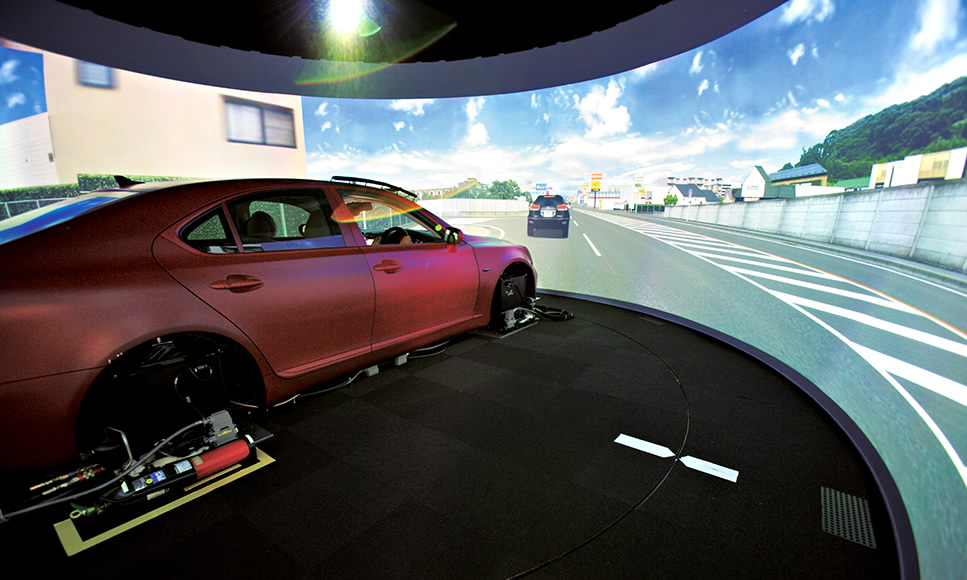
\includegraphics[width=0.9\linewidth]{./figures/ch3/driving_simu}}
    \caption{}
    \label{Fig:driving_simu}
  % \hspace{0.3cm}
  \end{subfigure}
  \begin{subfigure}{.4\textwidth}
  \centering
  {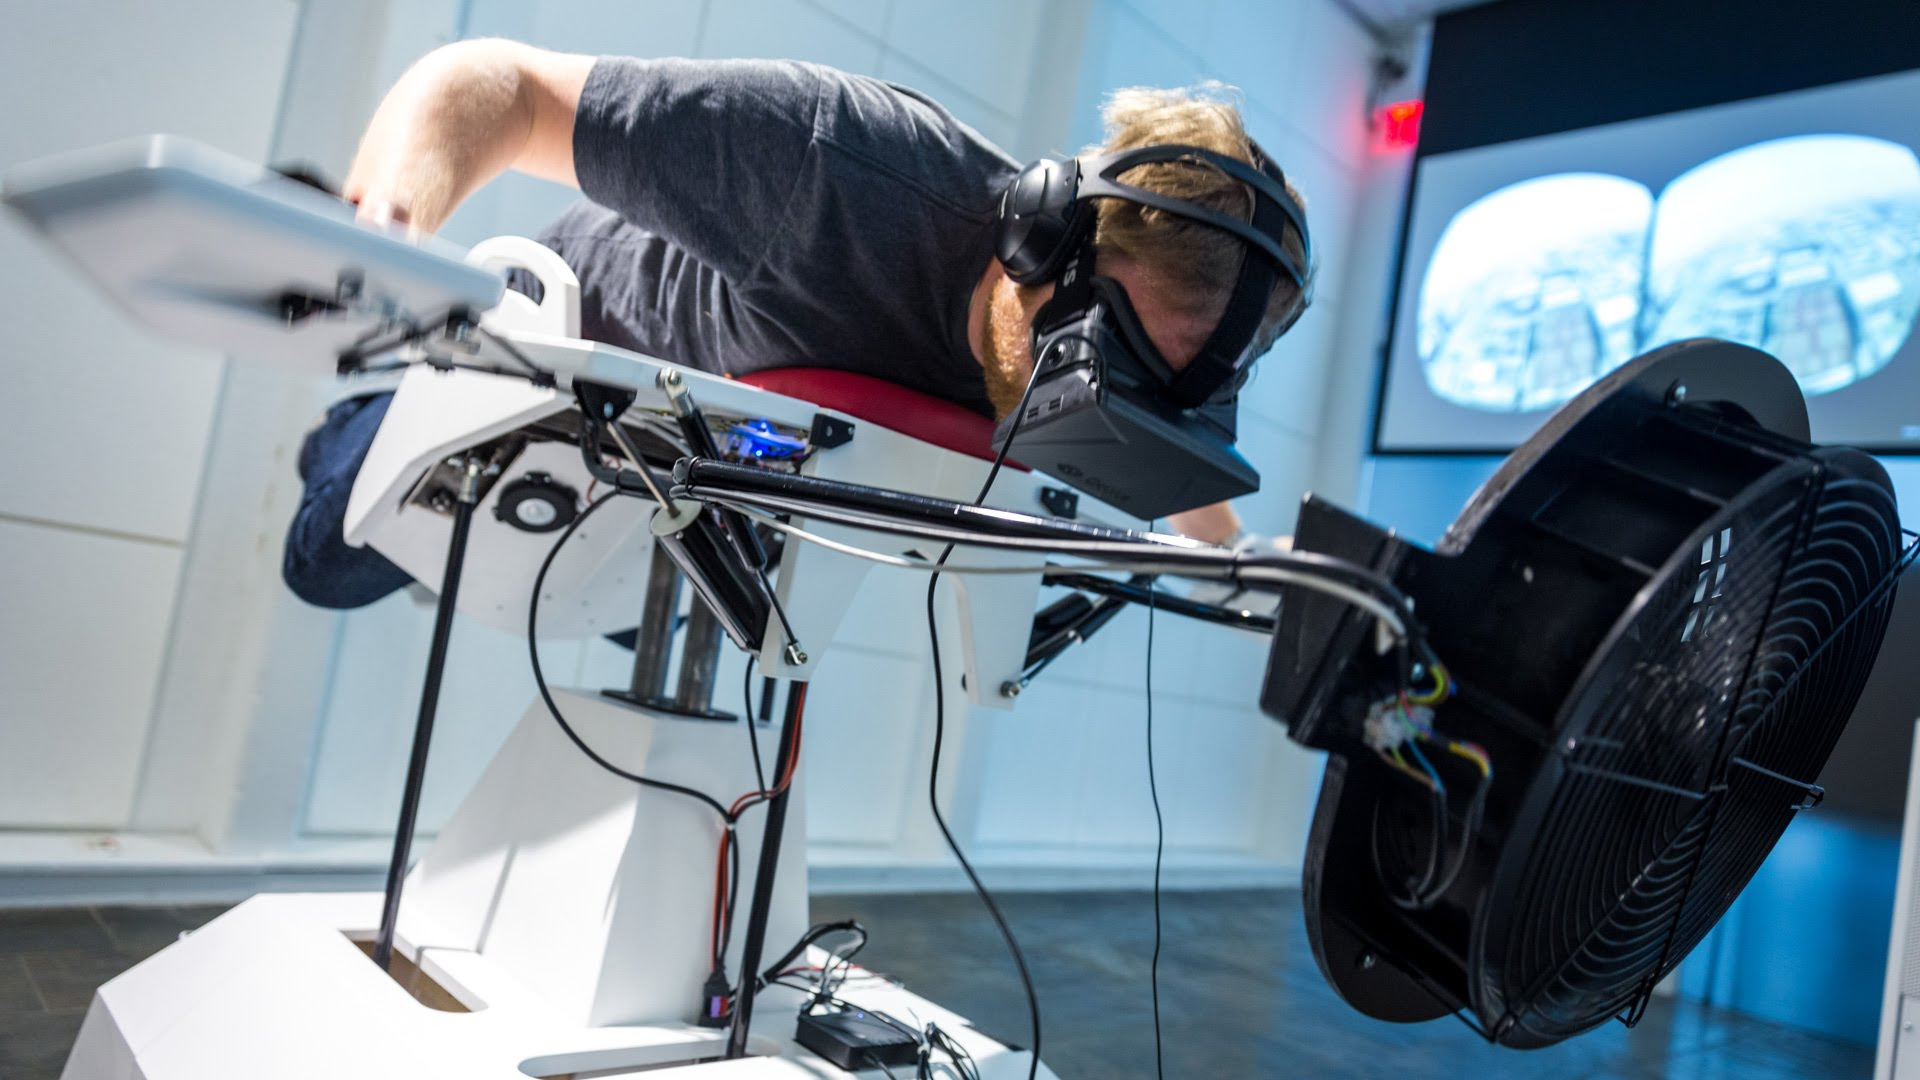
\includegraphics[width=0.7\linewidth]{./figures/ch3/flight_simu}}
    \caption{}
    \label{Fig:flight_simu}
  \hspace{0.3cm}
  \end{subfigure}
  \caption{\it (a) Exemple d'un simulateur de vol où les déplacements virtuels sont la conséquences des mouvements réels de l'utilisateur adoptant une posture de chute libre.
  (b) Simulateur de conduite dans un système de rétroprojection sur écran courbé.
  }
  % \hspace{0.3cm}
\end{figure}

\subsection{Méthodes de navigation dans des scènes virtuelles abstraites}

Conçus autour de contenus réalistes, les paradigmes cités précédemment sont néanmoins transposables à l'identique dans des scènes abstraites. Leur efficacité est cependant limité du fait de la nature différentes des données à observer. Alors que la navigation aura tendance à permettre l'exploration d'une surface virtuelle horizontale relativement étendue dans des scènes réalistes, les scènes abstraites scientifiques, et plus particulièrement les scènes moléculaires, concentrent les informations dans une zone centrale autour de laquelle l'utilisateur va évoluer. L'échelle de visualisation des données est capable d'augmenter la distance (toujours à l'échelle) des données observées mais la nature même de l'exploration est souvent différente. Sheidermann décrit la visualisation de données comme un processus où l'exploration est l'étape préliminaire avant les étapes de zoom et de filtre qui précèdent elle-même l'étape finale de l'obtention des détails à la demande. Les différentes échelles de précision mises en avant dans cette description sont rarement retrouvées dans les paradigmes de navigation au sein de scènes virtuelles réalistes.

Bien qu'il existe de nombreux portages de logiciels experts de visualisation moléculaire dans des EV, la navigation au sein de données scientifiques dans ces derniers s’inspire encore largement de la manipulation d'objet retrouvé dans les logiciels de visualisation moléculaire courants (voir Figure \ref{Fig:pymol_nav}). La manipulation d'objets n'est cependant pas adaptée aux environnements virtuels. Le nombre et la complexité des tâches de manipulation sont trop nombreuses pour s'adapter aux EV 3d qui favorisent des paradigmes de navigation simplifiées. La taille des objets, dont l'ordre de grandeur est ramené à la taille humaine pour une meilleure immersion, est un second frein à l'approche par manipulation. Elle favorise en effet la perte du peu de repères spatiaux que pouvaient posséder l'utilisateur, ces repères étant souvent limités au seul objet intérêt, l'environnement (skybox, paysage, etc.) étant majoritairement vide (voir \ref{}).   

\begin{figure}[h]
  \begin{subfigure}{.5\textwidth}
  \centering
  {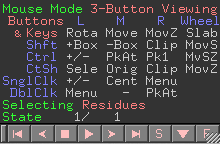
\includegraphics[width=0.9\linewidth]{./figures/ch3/pymol_nav}}
    \label{Fig:pymol_nav}
  % \hspace{0.3cm}
  \end{subfigure}
  \begin{subfigure}{.4\textwidth}
  \centering
  {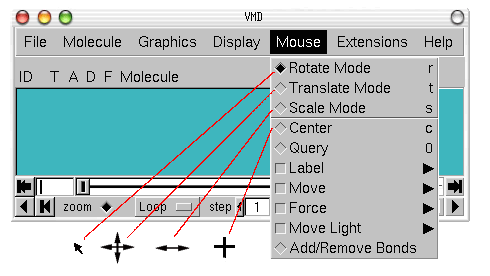
\includegraphics[width=0.7\linewidth]{./figures/ch3/vmd_nav}}
    \label{Fig:vmd_nav}
  \hspace{0.3cm}
  \end{subfigure}
  \caption{\it Capture d'écran des interfaces de manipulation offerts par PyMol (à gauche) et VMD à droite. Ils sont constitués de nombreuses combinaisons souris/clavier pour permettre d'utiliser l'ensemble des possibilités de manipulation disponibles.
  }
  % \hspace{0.3cm}
\end{figure}

Les seules tâches de navigation pouvant être identifiées au sein de logiciels experts de visualisation moléculaire se rapporte à des transitions progressives permettant de rejoindre une position spécifique depuis la position actuelle de l'utilisateur. Enfin, ces logiciels ne présentent aucune adaptation de la manipulation suivant le type de molécule observé et les paradigmes mis en jeu sont les mêmes que l'objet observé soit une protéine de quelques acides aminés ou bien un virus de plusieurs millions d'atomes. Dans tous les cas ils permettent une navigation totalement libre autour de la molécule et n'imposent aucune contrainte, au détriment de la conscience spatiale de l'utilisateur.

\section{Nouveaux paradigmes pour la RV}

Nous avons mis en évidence le besoin de mettre en place des paradigmes de navigation qui répondent aux problématiques posées par la visualisation moléculaire qui met en jeu des objets scientifiques abstraits, de plus en plus complexes, dans des environnements présentant un nombre réduit de repères spatiaux pour l'utilisateur.
